\part{Fault tolerance}
Four sources of faults in embedded systems:
\begin{enumerate}
    \item Inadequate specification, i.e. misunderstanding the interactions between the program and environment.
    \item Design errors in software components. We typically don't know the consequences of these.
    \item Failure of hardware components. More predictable than the one above.
    \item Interference in the supporting communication subsystem.
\end{enumerate}

\section{Reliability, failure and faults}
\textbf{Reliability} is a measure of how well a system conforms to the specification of its behavior. \emph{Response times} are an important part of the specification. \textbf{Failure} is when a system deviates from the specification. Highly reliable $\iff$ low failure rate.

The above definitions are concerned with the systems behaviour (external appearance). Failure stems from internal errors, whose algorithmic or mechanical causes are called \textbf{faults}. This motivates the following definition of a faulty component: A faulty component is one that under certain circumstances, during the lifetime of the system, results in an error.

An external state that is not in the specification is regarded as a failure, and an internal state that that is not specified is called an error. A fault is \textbf{active} when it produces an error, otherwise it is \textbf{dormant}. The error propagates through the system, and manifests itself as part of the external behavior.

A failure in one (sub)system can cause faults in other systems, as the following chain of events illustrates:\\
Fault $\xrightarrow{\text{activation}}$ Error $\xrightarrow{\text{propagation}}$ Failure $\xrightarrow{\text{causation}}$ Fault\\

With regard to time, there are three kinds of faults:
\begin{enumerate}
    \item \textbf{Transient faults} occur at some point in time, then disappear at some later point in time. E.g. HW response to external electromagnetic field, fault disappears when the field disappears. Common kind of fault in communication systems.
    \item \textbf{Permanent faults} start at a particular time, then remain in the system until they are fixed. E.g. SW design error.
    \item \textbf{Intermittent faults} are transient faults that occur from time to time, common with e.g. heat sensitive HW.
\end{enumerate}
\textbf{Bugs} are software faults, and originally there were two kinds:
\begin{itemize}
    \item \textbf{Bohrbugs} are reproducible and identifiable, can be removed during testing or with design diversity techniques.
    \item \textbf{Heisenbugs} are only active under certain rare circumstances, and often disappear when investigated. An example is code shared between concurrent tasks that is not properly synchronized. Heisenbugs can result from software ageing, e.g. not freeing allocated memory, and exhausting the available memory after a long time. Restarting the system clears this bug.
\end{itemize}

\section{Failure modes}
A system provides services, and its failure modes can be classified according to their impact on these services. Two general classes:
\begin{itemize}
    \item \textbf{Value failure} - Error in the value associated with service. Can be the result of a data conversion, e.g. 64-bit to 8-bit.
    \item \textbf{Time failure} - Service not delivered at the correct time.
\end{itemize}
Combinations of the two are called \emph{arbitrary} failures. Time failures can result in the service being delivered:
\begin{itemize}
    \item too early
    \item too late (performance error)
    \item infinitely late (omission failure) 
\end{itemize}
How can a system fail?
\begin{enumerate}
    \item Fail uncontrolled - arbitrary errors
    \item Fail late - delivers service too late in the time domain
    \item Fail silent - ommision failure
    \item Fail stop - same as above, but permits other systems to detect that it has failed silently
    \item Fail controlled - fails in a specified controlled manner
    \item Fail never - self explanatory
\end{enumerate}

\section{Fault prevention and fault tolerance}
\textbf{Fault prevention} aims to eliminate any and all faults before the system goes into operation, whilst \textbf{fault tolerance} enables the system to continue functioning even in the presence of faults. Both approaches attempt to give the system well-defined failure modes.

\subsection{Fault prevention}
Two steps; fault avoidance and fault removal. Fault avoidance consists of:
\begin{itemize}
    \item Acquiring reliable hardware and protecting it against interference.
    \item Rigorous specification of requirements, design based on e.g. UML (avsky).
    \item Use languages with data abstraction and modularity, like Ada and Java.
\end{itemize}
Fault removal consists of removing causes of errors, mainly by systems tests. However, testing can never remove all potential faults:
\begin{itemize}
    \item A test can only show the presence of faults, not their absence.
    \item It might be impossible to test under realistic conditions.
    \item Errors from the requirement analysis might not become visible until the system is in operation.
\end{itemize}
Any system will fail eventually (HW or SW), and for real-time systems we need fault tolerance.

\subsection{Fault tolerance}
Three levels of fault tolerance:
\begin{enumerate}
    \item \textbf{Full fault tolerance} - operation continues without significant loss of performance, but only for a limited time.
    \item \textbf{Fail soft} - operation continues, but a partial degradation in performance is accepted until recovery or repair.
    \item \textbf{Fail safe} - the system's integrity is maintained, but a temporary halt in operation is accepted. I.e. the system is shut down in a safe state. 
\end{enumerate}
Back in the day fault-tolerant design was based on three assumptions:
\begin{enumerate}
    \item Algorithms are correctly designed.
    \item All failure modes are known.
    \item All possible interactions with the environment are known.
\end{enumerate}
This is not realistic today, with multi-core processors and such, hence both anticipated and unanticipated errors must be accounted for.

\subsection{Redundancy}
\textbf{Protective redundancy} introduces components that detects and recovers the systems from faults, but are unnecessary for normal operation. When designing a fault-tolerant system, the goal is to minimize redundancy while maximizing reliability, subject to constraints on cost, size and power consumption. The redundant components can (and will) increase complexity, and it is useful to separate them from the rest of the system. 

We separate between static and dynamic redundancy, both for hardware and software. First, let's have a look at hardware redundancy:
\begin{itemize}
    \item \textbf{Static redundancy} (or masking) is based on redundant components ``hiding'' faults. An example is Triple Modular Redundancy (TMR), where a majority voting circuit is used. The output of three identical components are compared, and if one differs from the others, its output is masked out. It is assumed that faults are transient.
    \item \textbf{Dynamic redundancy} is an error-detection facility within a component, making it possible for that component to indicate if its output is in error. Note that the component does not hide or fix the error, that must be done by some other part of the system. Examples are checksums (see parity byte section on Wikipedia for very simple example) and parity bits.
\end{itemize}

For fault tolerance with regards to software design, we have \emph{N-version programming} which works like masking, and \emph{error detection and recovery}. The latter is dynamic redundancy in the sense that recovery is only brought into action once an error has occured.

\section{N-version programming}
From one initial specification, N independent programs are created. In operation, they run concurrently, and their outputs are compared by a driver process. The ``correct'' result is determined by majority of vote, like with masking. Challenges concerning N-version programming are:
\begin{itemize}
    \item \textbf{Initial specification} - It is close to impossible to produce unambiguous specifications.
    \item A complex part of the specification can potentially induce faults for all the N independent developer teams.
    \item Budget concerns, N-versions are N times more expensive than one.
    \item \textbf{Granularity} - How often results are compared affects overhead in one direction, and fault tolerance in the other.
    \item \textbf{Inexact voting} - Results may not agree exactly, even when no fault has occured. This is a consequence of \emph{finite-precision} arithmetic and the possibility of multiple correct solutions (a quadratic eq. being a simple example). One solution is to regard values inside a range of $\Theta$ to be equal, but then the problem arises once again for values close to the boundaries of the range.
\end{itemize}

\section{Software dynamic redundancy}
Statically redundant components operate whether or not an error has occured. With dynamic redundancy, however, the redundant components are only put into play when an error occurs. There are four phases to dynamic redundancy in software:
\begin{enumerate}
    \item \textbf{Error detection}
    \item \textbf{Error diagnosis} - There is a delay between a fault becoming active and error detection, the propagation of erroneous information in the system is assessed.
    \item \textbf{Error recovery} - Transform the corrupted system into a state where it can continue operation.
    \item \textbf{Fault treatment} - Maintenance must be performed to correct the underlying fault responsible for the error.
\end{enumerate}

\subsection{Error detection}\label{sec:error_detection}
There are two classes:
\begin{itemize}
    \item \textbf{Environmental detection} - Detection by hardware (e.g. overflow error) or run-time support system (e.g. out of bounds error for array).
    \item \textbf{Application detection}
    \begin{itemize}
        \item \textbf{Replication checks} - Check if results are equal for duplicate threads or processors (like N-version programming).
        \item \textbf{Timing checks} - Can be a \emph{watchdog timer} that has to be reset with a given frequency, or detection of missed deadlines by the scheduling system.
        \item \textbf{Reversal checks} - Compute the input from the output, and compare with the actual input.
        \item \textbf{Coding checks} - E.g. checksum
        \item \textbf{Reasonableness checks} - \texttt{assert()}-function
        \item \textbf{Structural checks} - E.g. count number of elements in list to confirm integrity.
        \item \textbf{Dynamic reasonableness checks} - Error assumed if new output is too different from previous value.
    \end{itemize}
\end{itemize}

\subsection{Error diagnosis}
Software designers aim to minimize the damage caused by a faulty component, this is called \emph{firewalling}. Two techniques are: 
\begin{itemize}
    \item \textbf{Modular decomposition} - Modules only communicate through well-defined interfaces, internal details are hidden. Provides a static structure.
    \item \textbf{Atomic actions} are indivisible, and appear to happen instantaneously for the rest of the system. Often called \textbf{transactions} or atomic transactions. They are used to move the system from one consistent state to another, and limit the flow of information between components/modules.
    \item There are also \textbf{protection mechanisms} which may stop a process from accessing a resource based on its access permissions.
\end{itemize}

\subsection{Error recovery}
There are two approaches; \textbf{forward} and \textbf{backward} error recovery.

Forward error recovery tries to continue from an erroneous state by finding a new consistent (but probably sub-optimal) state.  An example is Hamming codes (haven't read about them). Useful if the error related to the previous state may happen many times in a row, and one cannot afford to return to that state.

Backward error recovery restores the system to a previous safe state, a \textbf{recovery point}, and executes a different code block than the one that lead to an error. The new code should have the same functionalty, but use a different algorithm. Setting up a recovery point is called \textbf{checkpointing}.

Backward recovery can be used to recover from unanticipated faults (very good), but cannot undo effects the fault had on the environment (e.g. launching a missile). Furthermore, it may be costly in a real-time sense to save state from time-varying sensor data.

State restoration with concurrent processes is not necessarily simple, as is seen from the \textbf{domino effect}. Let us say we have two processes, say $P_1$ and $P_2$ that communicate, synchronize and set up recovery points. If $P_1$ detects an error at time $T_e$, it will roll back to its previous safe state. But what if there was communication between $P_1$ and $P_2$ between that state and $T_e$? Then $P_2$ must also roll back to its previous state, and there might have been some communication in between there as well. This might continue until both processes are back to square one, and is called the \emph{domino effect}. 

The probability of the domino effect increases with the number of concurrent processes. A \textbf{recovery line}, a consisent set of recovery points, is required to avoid the effect.

\section{Recovery blocks}
\Cref{fig:recovery_block} illustrates a recovery block.
\begin{figure}
    \centering
    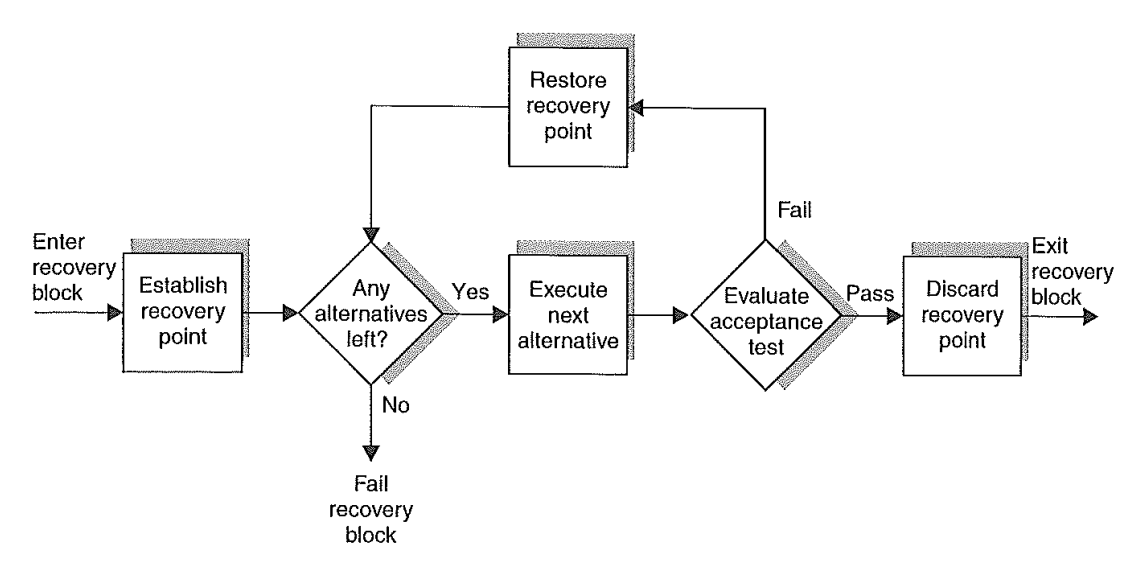
\includegraphics[width=0.8\textwidth]{figures/recovery_block.png}
    \caption{Structure of a recovery block.}
    \label{fig:recovery_block}
\end{figure}

\subsection{Acceptance test}
The acceptance test provides an error detection mechanism, e.g. with invokations of \texttt{assert()}. There is always a trade-off between a comprehensive test and affecting the 'happy path' as little as possible. All the error detection techniques discussed in \Cref{sec:error_detection} can be used to create acceptance tests.

Acceptance tests do not focus on specific error situations and error returns, since these will never handle unexpected errors.Instead we put demands on the current state to be acceptable.

\section{Comparison between N-version programming and recovery blocks}
Brief comparison:
\begin{itemize}
    \item N-version is static, all versions run regardless of whether an error has occured or not. Recovery blocks are dynamic.
    \item N-version requires a driver process, while recovery blocks need an acceptance test. At run-time N-version requires N times the resources, since recovery blocks only run one code block at a time. However, establishing recovery points, and reverting to them is expensive.
    \item Both are prone to errors stemming from ambiguous specifications.
    \item Acceptance tests may be more flexibe than e.g. an inexact voting scheme. 
    \item The backward error recovery of recovery blocks cannot undo effects on the environment (not impossible to design a system that avoids this problem), whereas N-version requires everything to go through the driver before it can affect the outside world.
\end{itemize}

\section{Dynamic redundancy and exceptions}
\textbf{Exception} $:=$ the occurence of an error. Telling the 'invoker' about the error condition is called \textbf{raising} (or signaling or throwing) and exception, and the invoker then \textbf{handles} (or catches) the exception. 

Exceptions can be regarded as forward error recovery, as the state is not rolled back, but control is handed over to the exception handler (still, backward recovery can be implemented with exceptions). There is an example in B\&W that illustrates some of the controversy surrounding exceptions.